\documentclass{beamer}
%\usepackage{fullpage}
%\usepackage[left=2.8cm,right=2.2cm,top=2 cm,bottom=2 cm]{geometry}
\setbeamersize{text margin left=10pt,text margin right=10pt}
\usepackage{amsmath,amssymb}             % AMS Math
\usepackage[T1]{fontenc}
\usepackage[utf8]{inputenc}
\usepackage[french,english]{babel}
\usepackage{txfonts} 
\usepackage[]{graphicx}
\usepackage{multirow}
\usepackage{hyperref}

%\renewcommand{\baselinestretch}{1.5}

\def\supit#1{\raisebox{0.8ex}{\small\it #1}\hspace{0.05em}}

\title[Vers une amélioration \\des résumés automatiques de textes \hspace*{2cm}  \textbf{\footnotesize  \insertframenumber/\inserttotalframenumber} ] %
{Vers une amélioration \\des résumés automatiques de textes} %:\\ Une méthode de score en utilisant le regroupement et l'apprentissage}
\institute{ %
École  nationale Supérieure d'Informatique (ESI, ex. INI), Algérie  %\\\supit{b} CERIST - Algérie %
}
\author[ARIES Abdelkrime (ESI 2014)] %
{ARIES Abdelkrime \\ {\footnotesize %
Encadré par: Pr. ZEGOUR Djamal Eddine\\%
Co-encadré par: Pr. HIDOUCI Khaled Walid}}

\titlegraphic{
\includegraphics[height=1cm]{IMG/esi-logo.png}%\hspace*{4.75cm}~
}

\date{État d'avancement deuxième année: 2014/2015} %\today

\usetheme{Warsaw} % Antibes Boadilla Warsaw

\beamertemplatenavigationsymbolsempty


\begin{document}

\selectlanguage {francais}

\begin{frame}[plain]
\maketitle
\end{frame}


\begin{frame}
\frametitle{Plan}
{\footnotesize \tableofcontents[hideothersubsections]}
\end{frame}

\section{Problématique}
\begin{frame}
\begin{center}
{\Huge Problématique}
\end{center}
\end{frame}

\subsection{Introduction}

\begin{frame}
\frametitle{Motivation}

\begin{itemize}
\item Augmentation du contenu dans le web,
\item Plusieurs sources et langues 
\end{itemize}
$ \Rightarrow $
\begin{itemize}
\item Utilisation de résumé automatique
\item Workshop pour le résumé automatique (ex. workshop "MultiLing" )
\end{itemize}

\end{frame}

\subsection{Description du problématique}

\begin{frame}
\frametitle{Problématique}

\begin{itemize}
\item Les méthodes extractives résultent des résumés non cohérents
\item Les méthodes abstractives consomment beaucoup de ressources
\item L'utilisation de l'apprentissage entraîne la dépendance du système au langue et genre du corpus.
\end{itemize}

\end{frame}

\begin{frame}
\frametitle{Objectifs}

\begin{itemize}
\item Créer une méthode complètement multilingue.
\item Améliorer la solution proposée dans \cite{13-aries-al}.
\item Minimiser les problèmes de lisibilité et de cohérence pour le résumé résultant.
\end{itemize}
\end{frame}

\section{Notre système (All Summarizer)}
\begin{frame}
\begin{center}
{\Huge Notre système (All Summarizer)}
\end{center}
\end{frame}

\begin{frame}
\frametitle{Notre système (All Summarizer)}
\framesubtitle{Architecture générale}

\begin{center}
\includegraphics[width=100mm]{IMG/gnrl_arch.pdf}
\end{center}

\end{frame}

\subsection{Prétraitement}

\begin{frame}
\frametitle{Prétraitement}

\begin{center}
\scriptsize
%\setlength{\tabcolsep}{6pt}
\begin{tabular}{p{.25\textwidth}p{.15\textwidth}p{.5\textwidth}} 
\hline \hline
Prerocess task & Tools & Languages \\
\hline
\multirow{3}{2cm}{Sentence segmentation} & openNLP\tablefootnote{\url{https://opennlp.apache.org/}} & Nl, En, De, It, Pt, Th \\
\cline{2-3}
& JHazm\tablefootnote{\url{https://github.com/mojtaba-khallash/JHazm}} & Fa \\
\cline{2-3}
& Regex & The remaining \\
\hline
\multirow{3}{2cm}{Words tokenization} & openNlp & Nl, En, De, It, Pt, Th \\
\cline{2-3}
& Lucene\tablefootnote{\url{https://lucene.apache.org/}} & Zh, Ja \\
\cline{2-3}
& Regex & The remaining \\
\hline
\multirow{3}{2cm}{Stemming} & Shereen Khoja\tablefootnote{\url{http://zeus.cs.pacificu.edu/shereen/research.htm}} & Ar \\
\cline{2-3}
& JHazm & Fa \\
\cline{2-3}
& HebMorph\tablefootnote{\url{http://code972.com/hebmorph}} & He \\
\cline{2-3}
& Lucene & Bg, Cs, El, Hi, Id, Ja, No \\
\cline{2-3}
& Snowball\tablefootnote{\url{http://snowball.tartarus.org/}} & Eu, Ca, Nl, En (Porter), Fi, Fr, De, Hu, It, Pt, Ro, Ru, Es, Sv, Tr \\
\cline{2-3}
& / & The remaining \\
\hline \hline
\end{tabular}

\end{center}

\end{frame}

\subsection{Traitement}

\begin{frame}
\frametitle{Traitement}
\framesubtitle{Regroupement}
\begin{center}
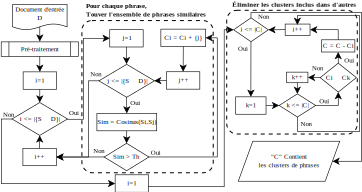
\includegraphics[width=9cm]{IMG/cluster.pdf}
\end{center}
\end{frame}

\begin{frame}
\frametitle{Traitement}
\framesubtitle{Apprentissage}
\[ P_{f}(f = \phi | c_j) = \frac {|\phi \in c_j|}{\sum_{c_l \in C}{|\phi' \in c_l|}} \]
$ f $: critère de sélection, $ \phi $: observation de $ f $, $ C $: ensemble de clusters.
\vfill
$ f \in $
\begin{itemize}
\item Fréquence des termes (unigram) (TFU)
\item Fréquence des termes (bigram) (TFB)
\item Position de la phrase (Pos)
\item Longueur de la phrase (Rleng, PLeng)
\end{itemize}
\end{frame}

\begin{frame}
\frametitle{Traitement}
\framesubtitle{Score des phrases}
\[ Score(s_i , c_j , f_k ) = 1 + \sum_{\phi \in s_i} {P(f_k=\phi | s_i \in c_j)} \]
\[ Score(s_i , \bigcap_{j} c_j , F) =  %\propto 
\prod_{j} \prod_{k} Score(s_i , c_j , f_k ) \]
\vfill
s: phrase, c: cluster, f: critère de sélection, F: ensemble des critères utilisées, $ \phi $: observation de $ f $.
\end{frame}

\subsection{Extraction}

\begin{frame}
\frametitle{Extraction}
\begin{center}
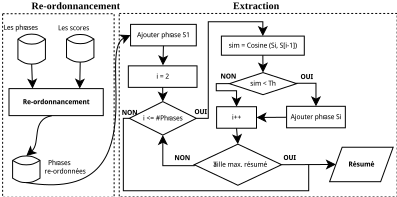
\includegraphics[width=11cm]{IMG/extract.pdf}
\end{center}
\end{frame}

\section{Nos contributions}

\begin{frame}
\begin{center}
{\Huge Nos contributions}\\
{\LARGE \textit{Notre travail pour l'année 2014/2015}}
\end{center}
\end{frame}

\subsection{Estimation des paramètres de résumé}

\begin{frame}
\frametitle{Estimation des paramètres de résumé}
\framesubtitle{Seuil de regroupemennt: mesures statistiques}
\begin{itemize}
\item La médiane
\item La moyenne arithmétique
\item Le mode: bas et haut.
\item La variance
\item $ sDn = \frac{\sum |s|}{|D| * n}$ 
\item $ Dsn = \frac{|D|}{n * \sum |s|}$ 
\item $ Ds = \frac{|D|}{\sum |s|}$ 
\end{itemize}
$|s|$: nombre de différentes termes dans une phrase $s$. 
$|D|$: nombre de différentes termes dans un document $D$.
$n$: nombre de phrases dans ce document.
\end{frame}

\begin{frame}
\frametitle{Estimation des paramètres de résumé}
\framesubtitle{La sélection des paramètres}
Tâche MMS - Corpus d'apprentissage - Anglais:
\begin{center}
\tiny
%\setlength{\tabcolsep}{6pt}
\begin{tabular}{p{.5cm}p{1cm}p{1cm}p{1cm}p{1cm}p{1cm}p{1cm}p{1cm}} 
\hline \hline

 & &  TFU-TFB-Pos-RLeng & TFU-TFB-Pos-PLeng & TFU-TFB-RLeng-PLeng & TFU-Pos-RLeng-PLeng & TFB-Pos-RLeng-PLeng & TFU-TFB-Pos-RLeng-PLeng\\
\hline
\multirow{8}{*}{M001} & median & 0.0909 & 0.1105 & 0.1259 & 0.1273 & 0.1385 & 0.0951\\
& sDn & 0.0783 & 0.0951 & 0.0895 & 0.1385 & 0.0951 & 0.1203\\
& Lmode & 0.1147 & 0.0937 & 0.1301 & \underline{0.1497} & 0.1245 & 0.0923\\
& Hmode & 0.1147 & 0.0937 & 0.1301 & \underline{0.1497} & 0.1245 & 0.0923\\
& mean & 0.0909 & 0.0909 & 0.1189 & 0.0923 & 0.1063 & 0.1357\\
& variance & 0.0783 & 0.0951 & 0.0895 & 0.1385 & 0.0951 & 0.1203\\
& Ds & 0.1119 & 0.1119 & 0.1063 & 0.1119 & 0.0531 & 0.1119\\
& Dsn & 0.0783 & 0.0951 & 0.0895 & 0.1385 & 0.0951 & 0.1203\\
\hline
\ldots &  &  &  &  &  & & \\
\hline 

\multirow{8}{*}{AVG} & median & 0.0105 & 0.0108 & 0.0112 & 0.0109 & 0.0122 & 0.0102\\
& sDn & 0.0075 & 0.0095 & 0.0111 & 0.0110 & 0.0093 & 0.0106\\
& Lmode & 0.0106 & 0.0099 & 0.0115 & 0.0133 & \textbf{0.0133} & 0.0100\\
& Hmode & 0.0125 & 0.0095 & 0.0115 & 0.0125 & 0.0114 & 0.0100\\
& mean & 0.0109 & 0.0089 & 0.0120 & 0.0097 & 0.0117 & 0.0133\\
& variance & 0.0075 & 0.0095 & 0.0111 & 0.0110 & 0.0093 & 0.0106\\
& Ds & 0.0091 & 0.0086 & 0.0099 & 0.0100 & 0.0100 & 0.0088\\
& Dsn & 0.0075 & 0.0095 & 0.0111 & 0.0110 & 0.0093 & 0.0106\\
\hline \hline
\end{tabular}

\end{center}
\end{frame}

\begin{frame}
\frametitle{Estimation des paramètres de résumé}
\framesubtitle{La sélection des paramètres}

\begin{center}
\scriptsize
\begin{tabular}{p{0.5cm}p{0.8cm}p{3cm}p{0.1cm}p{0.8cm}p{3cm}} 
\hline \hline

\multirow{2}{*}{Lang} & \multicolumn{2}{l}{Single document (MSS)} && \multicolumn{2}{l}{Multidocument (MMS)} \\

\cline{2-3} \cline{5-6} 
	& Th 		& Features 						&  & Th 	& Features \\
\hline
Ar 	& Ds 		& TFB, Pos, PLeng 				&  & Ds 	& TFB, Pos, RLeng, PLeng\\
Cs 	& HMode 	& TFU, TFB, Pos, PLeng 			&  & Ds 	& TFB, Pos, PLeng\\
El 	& Median 	& TFU, TFB, Pos, RLeng, PLeng 	&  & LMode 	& TFB, RLeng\\
En 	& Median 	& TFU, Pos, RLeng, PLeng 		&  & LMode 	& TFB, Pos, RLeng, PLeng\\
Es 	& sDn 		& TFB, PLeng 					&  & Ds 	& TFB, PLeng\\
Fr 	& Median 	& TFB, Pos, RLeng 				&  & Mean 	& TFU, TFB, Pos, PLeng\\
He 	& Ds 		& TFB, PLeng 					&  & Median & TFB, RLeng, PLeng\\
Hi 	& / 		& / 							&  & Ds 	& TFB, Pos, RLeng, PLeng \\
Ro 	& HMode 	& TFB, RLeng, PLeng 			&  & sDn 	& TFB, Pos, PLeng\\
Zh 	& HMode 	& TFB, RLeng, PLeng 			&  & sDn 	& TFU, Pos, RLeng, PLeng\\
\hline \hline
\end{tabular}

\end{center}
\end{frame}

\subsection{Participation à MultiLing'15 (SIGDIAL'15)}

\begin{frame}
\frametitle{MultiLing'15}
\framesubtitle{Critères de comparaison}

Soit AS = AllSummarizer\\
S = Un autre système qui a participé avec n langues\\

\[ AVG_{S} = \frac{\sum\limits_{i=1}^{n} Score_S(L_i)}{n} \]
\[ AVG_{AS} = \frac{\sum\limits_{i=1}^{n} Score_{AS}(L_i)}{n} \]

Amélioration relative (RI):
\[ RI = \frac{AVG_{AS} - AVG_{S}}{AVG_{S}} \]

\end{frame}

\begin{frame}
\frametitle{MultiLing'15}
\framesubtitle{Mono document (Tâche MSS)}
\begin{center}
\footnotesize
%\setlength{\tabcolsep}{6pt}
\begin{tabular*}{\textwidth}{@{\extracolsep{\fill}}lccccc} 
\hline \hline
\multirow{2}{*}{Methods} & \multicolumn{5}{c}{Our method improvement \%}\\
\cline{2-6}
							& ROUGE-1	& ROUGE-2	& ROUGE-3	& ROUGE-4	& ROUGE-SU4\\
\hline
BGU-SCE-M (ar, en, he)		& -09.19	& -14.02	& -19.39	& -25.12	& -11.07\\
EXB (all 38)				& -07.64	& -10.55	& -09.86	& -07.92	& -10.63\\
CCS (all 38)				& -07.33	& -13.24	& -10.95	& -03.04	& -07.40\\
BGU-SCE-P (ar, en, he)		& -04.33	& -01.63	& -02.69	& -06.16	& -01.89\\
UA-DLSI (en, de, es)		& +02.12	& +06.25	& +13.86	& +17.15	& +05.62\\
NTNU (en, zh)				& +06.44	& +07.06	& +11.50	& +21.81	& +05.74\\
\hline
Oracles (all 38) [TopLine]	& -31.64	& -49.00	& -63.80	& -72.91	& -36.77\\
Lead (all 38) [BaseLine]	& +02.39	& +08.67	& +08.20	& +04.02	& +05.82\\
\hline \hline
\end{tabular*}

\end{center}
\end{frame}

\begin{frame}
\frametitle{MultiLing'15}
\framesubtitle{Multidocument (Tâche MMS)}
\begin{center}
\footnotesize

%\setlength{\tabcolsep}{6pt}
\begin{tabular*}{\textwidth}{@{\extracolsep{\fill}}lcccc} 
\hline \hline
\multirow{2}{*}{SysID} & \multicolumn{3}{c}{Our method improvement \%}\\
\cline{2-4}
					& AutoSummENG 	& MeMoG 	& NPowER \\
\hline
UJF-Grenoble (fr, en, el) 	& -08.87 		& -14.55	& -03.62 \\
UWB (all 10) 		& -22.56 		& -22.66 	& -07.54 \\
ExB (all 10) 		& -09.44 		& -09.16 	& -02.80 \\
IDA-OCCAMS (all 10) 		& -17.11 		& -17.68 	& -05.53 \\
GiauUngVan (- zh, ro, es)	& -16.43		& -19.40	& -05.68 \\
SCE-Poly (ar, en, he)	& -05.72		& -03.35	& -01.46 \\
BUPT-CIST (all 10)		& +10.67		& +11.53	& +02.85 \\
BGU-MUSE (ar, en ,he)	& +05.67		& +06.92	& +01.74 \\
NCSR/SCIFY-NewSumRerank (- zh)		& +01.53		& -01.25	& +00.13 \\
\hline
our system (MSS parameters) (all 10)		& +01.98		& +02.35	& +00.58 \\
\hline \hline
\end{tabular*}

\end{center}
\end{frame}


\section{Conclusion et perspectives}
\begin{frame}
\begin{center}
{\Huge Conclusion et perspectives}
\end{center}
\end{frame}

\subsection{Conclusion}
\begin{frame}
\frametitle{Conclusion}
\begin{itemize}
\item Création d'une méthode multilingue
\item Estimer les paramètres (seuil et critères)
\item Tester le système par rapport aux systèmes récents (bonnes résultats) \cite{15-aries-al}.
\item Estimer les paramètres selon le document et sans prendre considération de la langue?
\end{itemize}
\end{frame}

\subsection{Perspectives}
\begin{frame}
\frametitle{Perspectives}
Pour cette année, notre but est:
\begin{itemize}
\item Estimer les paramètres pour chaque document et pas pour chaque langue.
\item Proposer une meilleure méthode pour la détection de similarité entre phrases.
\item Améliorer l’ordonnancement des phrases après l'extraction.
\item Améliorer la lisibilité du résumé généré (Anglais comme langue de début):
\begin{itemize}
\item Couramment, on travaille sur une méthode pour représenter les phrases, en tenant compte de l'aspect multilingue.
\item On a proposé une structure (partielle) basée sur JSON pour représenter les phrases.
\end{itemize}
\end{itemize}
\end{frame}

\begin{frame}
\frametitle{Fin ...}

\begin{center}
{\Huge Merci pour votre attention}
\end{center}
\end{frame}


%\subsection{Bibliography}
\frame[allowframebreaks]%
{\frametitle{Bibliography}
\tiny
\bibliography{biblio}
\bibliographystyle{IEEEtran} 
}


\end{document}

